\documentclass[border=2pt]{standalone}
\usepackage{amsmath}
\usepackage{tikz}
\usetikzlibrary{intersections}
\usetikzlibrary{arrows}
\usetikzlibrary{quotes,angles}
\usepackage{amsmath}
\usepackage{xcolor}

\begin{document}

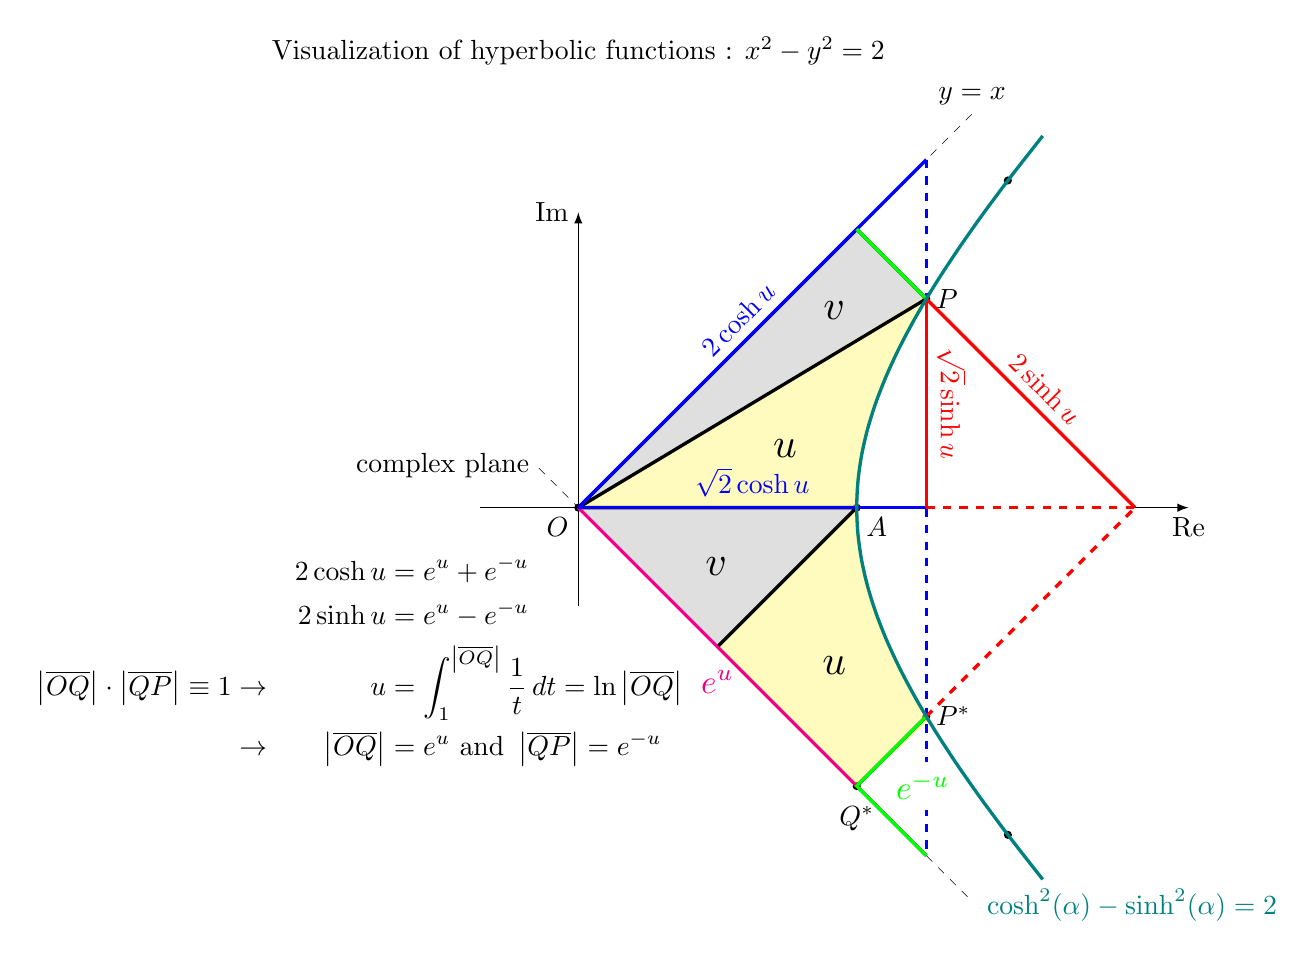
\begin{tikzpicture}[scale=2.5]

% Draw x and y axis lines
\draw [->,>=latex] (-0.5,0) -- (3.10,0) node [below] {$\mathrm{Re}$};
\draw [->,>=latex] (0,-0.5) -- (0,1.50) node [left ] {$\mathrm{Im}$};
\node[above left] at (-0.2, 0.1) {complex plane};
%\filldraw[black] (1,0) circle (0.5pt) node[below right] {$1$} ;
%\filldraw[black] (0,1) circle (0.5pt) node[above right] {$j$} ;
\node[above] at (0.0,2.2) {Visualization of hyperbolic functions : $x^2 - y^2 = 2$};

% Draw a circle at the origin of radius 1
%\draw (0,0) circle (1);

\draw [very thin, dashed] (-0.0,-0.0) -- ( 2.0, 2.0) node[above] {$y=x$} ;
\draw [very thin, dashed] (-0.2, 0.2) -- ( 2.0,-2.0) ;

\pgfmathsetmacro{\angle}{1.0}
\pgfmathsetmacro{\length}{\angle}
\pgfmathsetmacro{\scale}{sqrt(2)}

\filldraw[black] ( 0.0, 0.0) circle (0.5pt) node[below left] {$O$} ;
%\filldraw[black] ( 0.5*\scale, 0.5*\scale) circle (0.5pt) node[above=2pt ] {$B$} ;
%\filldraw[black] ( 0.5*\scale,-0.5*\scale) circle (0.5pt) node[below=4pt ] {$B^*$} ;
\filldraw[black] ({sqrt(2)}, 0) circle (0.5pt) node[below right] {$A$} ;
\filldraw[black] ({ 2.5/\scale}, { 1.5/\scale}) circle (0.5pt) node[right ] {$P$} ;
\filldraw[black] ({ 2.5/\scale}, {-1.5/\scale}) circle (0.5pt) node[right ] {$P^*$} ;
%\filldraw[black] ({ 1.0*\scale}, { 1.0*\scale}) circle (0.5pt) node[right=2pt ] {$Q$} ;
\filldraw[black] ({ 1.0*\scale}, {-1.0*\scale}) circle (0.5pt) node[below=4pt ] {$Q^*$} ;

\draw [thick, draw=gray,fill=gray!50,opacity=0.5] ( 0.0, 0.0) -- ( 1.0*\scale, 1.0*\scale) -- ({ 2.5/\scale}, { 1.5/\scale}) -- ( 0.0, 0.0) -- ({ 2.5/\scale}, { 1.5/\scale}) ;
\draw [thick, draw=gray,fill=gray!50,opacity=0.5] ( 0.0, 0.0) -- ( {sqrt(2)}, 0.0) -- ( 0.5*\scale,-0.5*\scale) -- ( 0.0, 0.0) -- ( 0.5*\scale,-0.5*\scale) ;
\node [scale=1.5] at ( 1.30, 1.00) {$v$} ;
\node [scale=1.5] at ( 0.70,-0.30) {$v$} ;

\draw[very thick,smooth, draw=yellow,fill=yellow!50,opacity=0.5, variable=\x] plot[domain= 0.5*\scale:0] ({ cosh(\x)*\scale}, {sinh(\x)*\scale}) -- ( 0.0, 0.0) ;
\draw[very thick,smooth, draw=yellow,fill=yellow!50,opacity=0.5, variable=\x] plot[domain=-0.5*\scale:0] ({ cosh(\x)*\scale}, {sinh(\x)*\scale}) -- ( 0.5*\scale,-0.5*\scale) -- ({ 1.0*\scale}, {-1.0*\scale}) ;
\node [scale=1.5] at ( 1.05, 0.30) {$u$} ;
\node [scale=1.5] at ( 1.30,-0.80) {$u$} ;

\draw[very thick] (0,0) -- ({ 1.0*\scale}, { 1.0*\scale}) -- ({ 2.5/\scale}, { 1.5/\scale}) -- (0,0) ;

\draw[very thick] (0,0) -- (\scale, 0) -- ({ 0.5*\scale}, {-0.5*\scale}) ;
\draw[very thick, magenta] (0,0) -- node[below=4pt, scale=1.2] {$e^u$} ({ 1.0*\scale}, {-1.0*\scale}) ;
\draw[very thick] ({ 1.0*\scale}, {-1.0*\scale}) -- ({ 2.5/\scale}, {-1.5/\scale}) ;

\draw [very thick,dashed, blue] ({ 2.5/\scale}, { 2.5/\scale}) -- ({ 2.5/\scale}, {-2.5/\scale}) ; 

\draw [very thick, blue] (0,0) -- node[above, rotate=45] {$2\cosh u$} ({ 2.5/\scale}, { 2.5/\scale}) ; 
\draw [very thick, black] (0,0) -- ({ 2.5/\scale}, 0) ; 
\draw [very thick, blue] (0,0) -- node[above] {$\sqrt{2}\cosh u$} ({ 2.5/\scale}, 0) ; 

\draw [very thick, green] ({ 2.5/\scale}, { 1.5/\scale}) -- ({ 1.0*\scale}, { 1.0*\scale}) ; 
\draw[very thick] ({ 1.0*\scale}, {-1.0*\scale}) -- ({ 2.5/\scale}, {-2.5/\scale}) ;
\draw [very thick, green] ({ 2.5/\scale}, {-1.5/\scale}) -- ({ 1.0*\scale}, {-1.0*\scale}) -- ({ 2.5/\scale}, {-2.5/\scale}) ; 
\node[right=10pt, green, scale=1.2,fill=white] at ({ 1.0*\scale}, {-1.0*\scale}) {$e^{-u}$} ;

\draw [very thick, white, opacity=1.0] ({ 2.5/\scale}, 0) -- (2 * \scale, 0) ; 
\draw [very thick, dashed, red] ({ 2.5/\scale}, 0) -- (2 * \scale, 0) ; 

\draw [very thick, white, opacity=1.0] ({ 2.5/\scale}, 0) -- ({ 2.5/\scale}, { 1.5/\scale}) ; 
\draw [very thick, red] ({ 2.5/\scale}, 0) -- node[above, rotate=-90] {$\sqrt{2}\sinh u$} ({ 2.5/\scale}, { 1.5/\scale}) ; 
\draw [very thick, red] ({ 2.5/\scale}, { 1.5/\scale}) -- node[above, rotate=-45] {$2\sinh u$} (2 * \scale, 0) ; 
\draw [very thick, dashed, red] ({ 2.5/\scale}, {-1.5/\scale}) -- (2 * \scale, 0) ; 

\filldraw[black] ({ cosh(\angle)*\scale}, { sinh(\angle)*\scale}) circle (0.5pt) ;
\filldraw[black] ({ cosh(\angle)*\scale}, {-sinh(\angle)*\scale}) circle (0.5pt) ;

%\draw[very thick] (0,0) -- ({ cosh(\angle)*\scale}, { sinh(\angle)*\scale}) ;
%\draw[very thick] (0,0) -- ({ cosh(\angle)*\scale}, {-sinh(\angle)*\scale}) ;



% 画双曲线
\draw[very thick,smooth,variable=\x, teal] plot[domain=-\angle-0.1:\angle+0.1] ({ cosh(\x)*\scale}, {sinh(\x)*\scale}) ;
\node[below right, teal] at ({ cosh(\angle-0.1)*\scale}, {-sinh(\angle+0.1)*\scale}) {$\cosh^2(\alpha) - \sinh^2(\alpha) = 2$} ;
%\draw[very thick,smooth,variable=\x, teal] plot[domain=-1.2:1.2] ({-cosh(\x)}, {sinh(\x)}) ;


%\draw[very thick, cyan] ({ cosh(\angle)*\scale}, {-sinh(\angle)*\scale}) -- ({ cosh(\angle)*\scale}, { sinh(\angle)*\scale}) ;

\node [below right] at (-2.8,-0.2) {
$
\begin{aligned}
 &  & 2\cosh u & =e^{u}+e^{-u}\\
 &  & 2\sinh u & =e^{u}-e^{-u}\\
\left|\overline{OQ}\right|\cdot\left|\overline{QP}\right|\equiv1 & \rightarrow & u & =\int_{1}^{\left|\overline{OQ}\right|}\frac{1}{t}\,dt=\ln\left|\overline{OQ}\right|\\
 & \rightarrow & \left|\overline{OQ}\right| & =e^{u}\ \text{and}\ \left|\overline{QP}\right|=e^{-u}
\end{aligned}
$} ;


\end{tikzpicture}

\end{document}
